% This file is isea.tex.  It contains the formatting instructions for and acts as a template for submissions to ISEA 2015.  It is based on the ICCC  formats and instructions.  It uses the files isea.sty, isea.bst and isea.bib, the first two of which also borrow from AAAI IJCAI formats and instructions.
% Modified from ICCC.tex by B. Bogart

\documentclass[letterpaper]{article}
\usepackage{isea}
\usepackage[pdftex]{graphicx}
\usepackage{times}
\usepackage{helvet}
\usepackage{courier}
\usepackage[numbers]{natbib}
\pdfinfo{
/Title (Scaling with multiple network namespaces in a single application)
/Author (PJ Waskiewicz)}
% The file isea.sty is the style file for ISEA 2015 proceedings.
%
\title{Scaling With Multiple Network Namespaces in a Single Application}
\author{PJ Waskiewicz\\
\\
NetApp\\
Portland, OR, USA\\
pj.waskiewicz@netapp.com\\
\newline
\newline
}
\setcounter{secnumdepth}{0}

\begin{document} 
\maketitle
\begin{abstract}
Namespaces and containers seem to be the rage today, but it’s not typical for large applications to use them directly. Rather, applications rely on frameworks such as LXC and/or Docker to manage the containers they run in.

This paper will focus on how a large application can utilize the network namespace framework, and how it can use large numbers of namespaces to partition up the underlying network infrastructure within the application. An overview of parts of the application architecture using the namespaces will be covered, showing the use cases driving the need for namespaces. Lessons learned around scalability and performance bottlenecks in the kernel will be shared.

Ultimately this paper will propose further improvements to the namespace framework for better programmatic management of namespaces within the kernel from userspace, as well as attention to increased scalability and efficiency of networking within the namespaces.
\end{abstract}

\section{Keywords}

networking, kernel, containers, namespaces, scaling, cloud

\section{Introduction}
The ongoing evolution of the datacenter towards cloud-based infrastructure continues to present interesting challenges to existing applications. These existing solutions, e.g. storage appliances, work to serve multiple tenants within a computing domain. However, when the infrastructure around these solutions evolves into a cloud-based, partitioned environment, these solutions must also evolve.

When an application has core logic that needs to span multiple, separate network environments, it must become container/network-namespace aware. The Linux kernel exposes an API to create and manage network namespaces within an application. This paper will focus on this API for the following:
\begin{itemize}
\item How to create and manage the lifecycle of a network namespace within a complex application
\item How to track and process multiple network connections across multiple network namespaces in an efficient and scalable manner
\item What limitations exist in this API that makes lifecycle management a challenge, along with proposals on how to improve the API for better lifecycle management
\item Scalability issues encountered, how these were addressed, and proposals around scalability testing to prevent regressions
\end{itemize}

\section{The Need For Multiple Network Namespaces}
Typical network-based storage applications have various layers of the core logic separated from one another. For example, the volume database containing metadata mappings to underlying block or object data is completely separated from the networking core, since they share no common functionality. In Figure \ref{app-overview}, one can see an example of how different components are separated from one another. Core logic for volume tracking in one functional area, thread management in another area, the iSCSI or Fibre Channel protocol stack handled elsewhere, and ultimately the underlying networking being handled by the underlying OS.

Consider a public or private cloud environment, where "legacy" datacenter models migrate pieces of their infrastructure into that cloud environment. A typical storage application as Figure \ref{app-overview} could have all storage volumes from that legacy datacenter migrated as one tenant. However, multiple tenants may have conflicting environment configurations, such as IP address range collisions, different routing hierarchies, or different VLAN segregation within their respective network domains. By creating a completely new network stack inside of a network namespace for each of these legacy environments, the containers can fully segregate the network environments from one another, and avoid any changes to the legacy datacenter configuration.

When an application architecture such as this needs to fit into an environment where the networking is the component that needs to support multiple containers, one can observe that using Docker or LXC is not sufficient. They are not sufficient since those deal with containerizing an entire application, not pieces of an application. Let us consider some different approaches to try and solve this problem of supporting multiple network stacks within an application.

\begin{figure}[h]
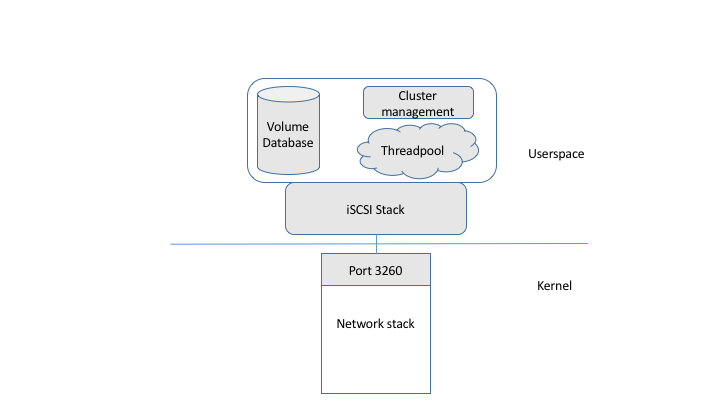
\includegraphics[width=3.31in]{standard-app-overview.png}
\caption{High-level architecture of application.}
\label{app-overview}
\end{figure}

\subsection{Approach 1: Fork application per-network namespace}
Each network namespace that is created within an application needs to have some mechanism to process traffic inbound and outbound to it. One approach is after creating the namespace and configuring it, fork() the application completely, and assign a fork()'d copy to each namespace configured.

This approach has serious limitations. As seen in Figure \ref{namespace-fork}, the core logic of the application needs to have added inter-process communication (IPC) to manage the non-networking pieces of the internals. This adds massive complexity, and impacts the entire application, instead of just the underlying networking pieces. In addition, applications like this are typically complex systems, and require significant system resources such as CPU and RAM. Having multiple copies of the entire application running on a system is completely infeasible.

\begin{figure}[h]
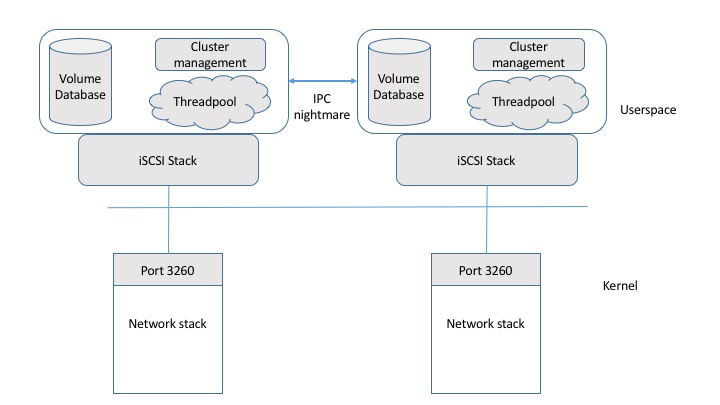
\includegraphics[width=3.31in]{multiple-stacks-no-namespace.png}
\caption{Multiple network namespaces with fork().}
\label{namespace-fork}
\end{figure}

\subsection{Approach 2: Thread per-network namespace}
A different approach post-namespace creation is to create a new thread (LWP) and assign it to the network namespace. This thread would then live in that network namespace context for its lifetime, and could process any inbound and outbound traffic to and from the namespace.

As seen in Figure \ref{namespace-threads}, this approach does not affect the core logic of the application. It only requires a new thread per-network namespace, and only affects the underlying networking core of the application. However, this approach does not scale well with large numbers of network namespaces. In highly complex applications that are multi-threaded, creating dedicated worker threads for specific tasks is usually not desirable. In addition, a single thread per-network namespace severely limits the processing capabilities of that network interface, especially if the underlying hardware is multiqueue-capable.

\begin{figure}[h]
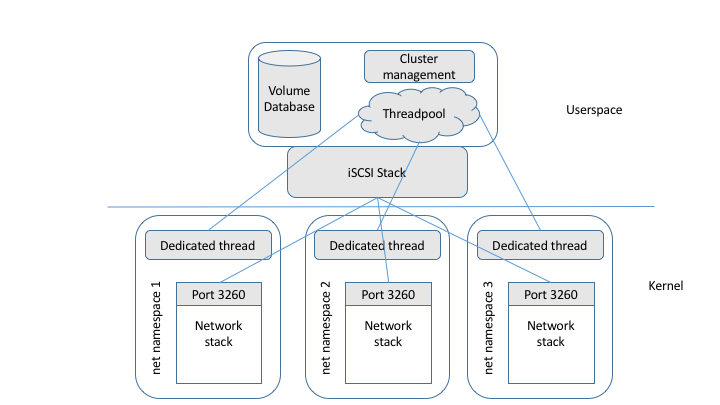
\includegraphics[width=3.31in]{multiple-stacks-namespaces-dedicated-threads.png}
\caption{Multiple network namespaces with dedicated threads.}
\label{namespace-threads}
\end{figure}

\subsection{Approach 3: Global file descriptor per-network namespace}
A final approach post-namespace creation is to switch a thread into the namespace, create a socket and bind the desired listening port inside of the namespace to that socket. Because file descriptors are not specific to each network namespace, all threads of our application have access to these file descriptors. When data needs to be read or written to a socket in a specific namespace, the currently-running thread can switch into that namespace context, and then access the socket using the global file descriptor.

As illustrated by Figure \ref{namespace-fds}, each network namespace stack opens port 3260 (iSCSI), and has a file descriptor that is unique to the system assigned to it. Then within the networking core of the application, the namespace that specific file descriptor belongs to is stored with the socket information, giving the core application logic the ability to switch in and out of each network namespace as needed. This does not require any additional threads or processing units, and can allow the core logic to be completely unaware of the underlying network segregation.

\begin{figure}[h]
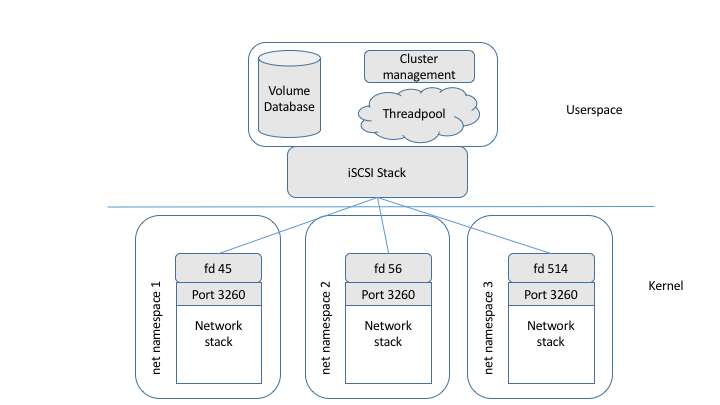
\includegraphics[width=3.31in]{multiple-namespaces-with-fd.png}
\caption{Multiple network namespaces with file descriptors.}
\label{namespace-fds}
\end{figure}

\section{Network Namespace Management}
Before diving into how to create and manage network namespaces inside of an existing application, one should understand how to interact with them at a basic level\cite{edge2014}. Once one is familiar with how to manage network namespaces from an administrative perspective, then diving into the programmatic side is the next logical step\cite{man2016}.

The biggest challenge with integrating network namespaces into an existing application is to manage their lifecycle efficiently. Things such as distinguishing newly-created network namespaces from recently destroyed network namespaces, how to switch into a namespace, and how to switch to the default/base namespace, are all things that need to be managed.

\subsection{Identifying Different Namespaces}
One challenge with network namespace management is how to distinguish a network namespace beyond just its name. Each network namespace is accessed by a file descriptor returned by opening /run/netns/\textit{namespace name} or by opening /proc/\textit{pid}/ns/net, where \textit{pid} is a process that currently lives inside that network namespace. In order for a complex application to have a chance at distinguishing between namespaces, one reference to each network namespace must be maintained for the life of that namespace; i.e. one file descriptor for each namespace must be maintained for all threads.

However, this isn't sufficient to uniquely identify one network namespace from another. If one network namespace is destroyed and another quickly created, the file descriptor returned from open(/run/netns/\textit{new namespace}); may be the same that was used to track the previously destroyed namespace. This can cause very unexpected results if the networking core of our application is only using file descriptors to track the namespaces.

If one adds one more piece of identification, then a "fairly" safe match can be made when comparing network namespaces. By adding the mtime of the kernel handle that /run/netns/\textit{namespace name} is backed by, this provides enough granularity that very quick destruction and addition of namespaces can be distinguished from one another. The mtime in this case is the same as when the special file was created, and is not updated by the kernel if changes are made to the namespace. This makes it a great candidate to help with unique indentification of each namespace along with its single file descriptor reference.

\subsection{Switching Threads Between Namespaces}
When using the approach in Figure \ref{namespace-fds} to create and manage network namespaces, it's very simple to switch into the namespace. A simple call to open() to get the file descriptor of the namespace is needed, then a call to setns() to switch. See Figure \ref{switch-new-namespace}. This will switch the current thread into the new namespace context, but it will also leave the thread in that context.
\begin{figure}[h]
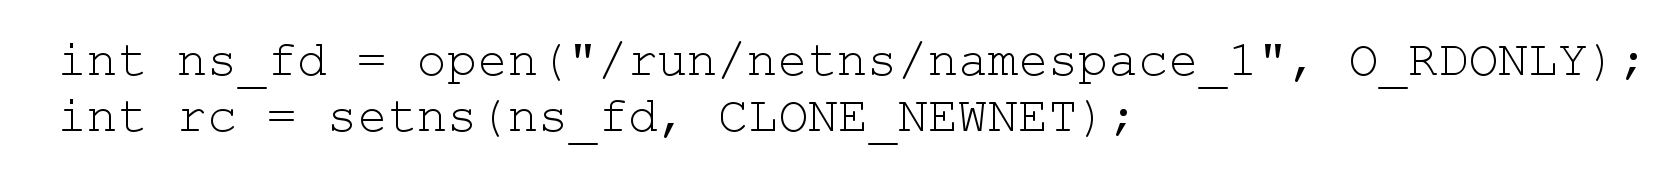
\includegraphics[width=3.31in]{switch-new-namespace.png}
\caption{Basic switching to new network namespace}
\label{switch-new-namespace}
\end{figure}

If the thread needs to be left in a known state, such as returning to the base or default namespace, then see Figure \ref{switch-base-namespace}. This assumes that PID 1 is in the default namespace of the kernel, or the default for the PID namespace if one is being used. If there's a different default/base namespace to return to, then one would cache a different PID's namespace file descriptor in the same fashion.
\begin{figure}[h]
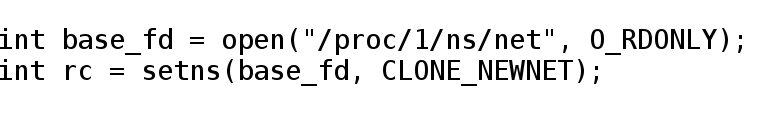
\includegraphics[width=3.31in]{switch-base-namespace.png}
\caption{Basic switching to default network namespace}
\label{switch-base-namespace}
\end{figure}

\subsection{Efficient Namespace Switching}
In order to utilize the same threadpool for any number of network namespaces, decisions need to be made when to switch between namespaces. If the application needs to incur the setns() system call for each network transaction in flight, the context switching can get very expensive, and is more than likely unnecessary. To make selective switching happen, one needs to cache a bit more information.

At this point, the application has cached the global file descriptor for each active network namespace, the global file descriptor for the base namespace, and what namespace each listening network port is assigned to. The last piece of information to cache is what namespace each thread is currently in. That can be stored inside thread-local storage (TLS) for each thread in the application. Using this information, when a socket operation needs to be performed, the namespace information can be pulled from the socket, and the current namespace of the thread in TLS can be compared to the socket's namespace. If they are the same, the setns() call can be avoided. Otherwise, the thread can be switched into that network namespace's context, and then the socket processing can continue.

\section{Network Namespace Scalability}
Making good decisions on when to switch a thread between namespaces is only part of the scalability story. The kernel itself also needs to be very efficient when dealing with any number of network namespaces, and how it performs the requested switch. We observed that in older 3.x Linux kernels, switching between namespaces had a massive performance impact. The latency of how long a switch took increased more than exponentially as more namespaces were added.  This was due to using RCU protection for the running task's nsproxy, versus using task\_lock() (i.e. a spin\_lock()). This was addressed in a patch by Eric Biederman \cite{biederman2014}, and had a drastic improvement in performance.

\begin{figure}[h]
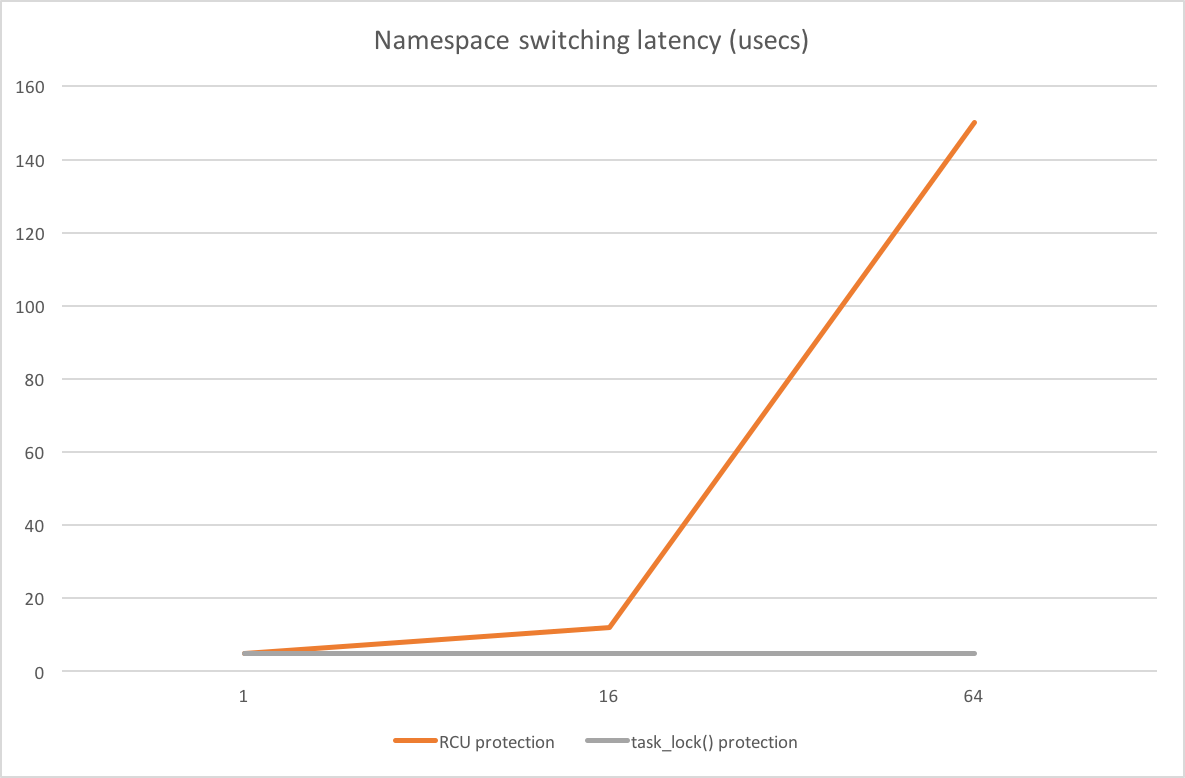
\includegraphics[width=3.31in]{close-up-latency.png}
\caption{Network namespace switching latency, close-up}
\label{close-latency}
\end{figure}

In Figure \ref{close-latency}, the namespace switching took 5 $\mu$secs with 1 network namespace, before and after the patch. However, approaching 64 network namespaces, pre-patch took an average of 150 $\mu$secs per switch, where post-patch it remained around 5 $\mu$secs. Expanding this out to 512 network namespaces, Figure \ref{full-latency} shows that the latency at 512 namespaces pre-patch took over half a second per switch, versus post-patch, the latency remains around 5 $\mu$secs.

\begin{figure}[h]
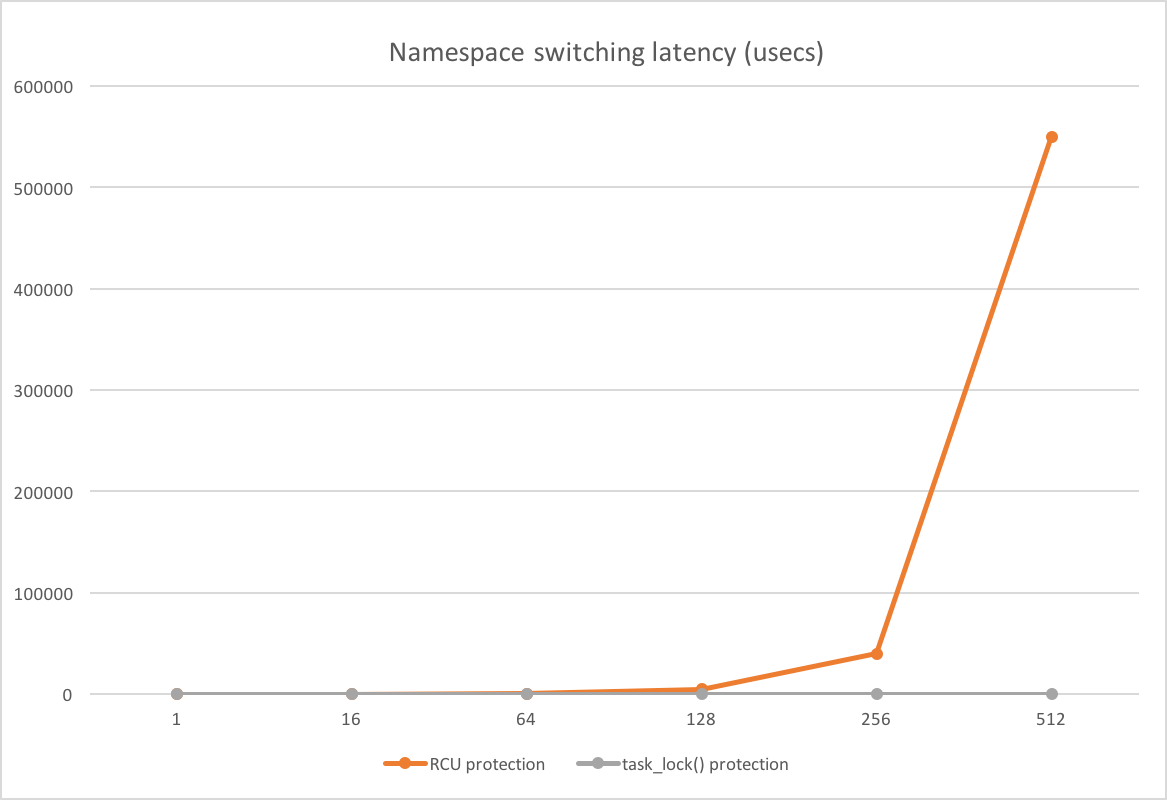
\includegraphics[width=3.31in]{full-namespace-latency.png}
\caption{Network namespace switching latency}
\label{full-latency}
\end{figure}

\section{Proposed Improvements}

\subsection{More Uniqueness}

\subsection{Performance Regression Testing}

\section{Conclusion}
The network namespace API in the Linux kernel provides a very powerful framework for applications to take advantage of. This allows large applications that need to span multiple network namespaces to not require complete architectural upheavals of core logic outside of the networking layers. Using some clever tricks and techniques, the namespace switching and lifecycle management can be very efficient. Moving forward, we believe there is still more that can be done to improve this API, and make it even more powerful as containers continue to grow in popularity and wide-spread deployment across the computing industry.

\section{Acknowledgments}
We would like to acknowledge the engineers who contributed to this network namespace application design: Carl Seelye, Marshall McMullen, Jared Cantwell, Tom Distler, and Joe Roback.

We would also like to acknowledge the Netdev1.2 selection committee for inviting us to submit and present this paper.

\bibliographystyle{pj-netdev-1.2}
\bibliography{pj-netdev-1.2}

\section{Author Biography}
PJ Waskiewicz is a Principal Software Engineer at NetApp in the SolidFire division. Prior to SolidFire/NetApp, PJ worked for many years as a network kernel engineer and device driver developer in the Networking Division of Intel. There he maintained and helped create the igb, ixgbe, and i40e wired Ethernet network drivers, the initial Tx multiqueue support in the Linux kernel network stack, and added Data Center Bridging support to the Linux kernel. He also worked in Intel's Open Source Technology Center on the x86 kernel tree, enabling advanced features in the Broadwell and Skylake microarchitectures.

\end{document}
